% !TeX root = repressed-anger.tex

\section{Sentiment Analysis}
\label{sec:sentiment_analysis}

\acrfull{sa}, sometimes referred as \acrfull{om}, is the field of study that aims determine the attitude of the author respect to some topic. During the last decade, due mainly to the rapid increase of the social media, the research of this area, which includes linguistics and \acrfull{nlp}, has gain more relevance as it has a wide range of applications that can be used commercially.

Almost the human actions are influenced by opinions. A practical example of this behavior that get repeated in daily basics occurs when before making a decision we want to know other' to contrast our thoughts. In business, when an organization requires to public or consumer opinion, it conducted different types of surveys to gather this information. However, nowadays we do not precise to ask personally to people around us to discuss about a product. Thanks to micro-blogs, Twitter and reviews in social networks, we can broaden the amount of external opinions for decision making. Due to the amusing amount of information available, sometimes we could face some challenges, such as finding reliable sources summarizing and filtering the relevant information. The same way we consume this information, companies also search for new ways to obtain and process such information efficiently without human intervention, to achieve this automated analysis is needed\cite{liu2012sentiment}.

\subsection{Tasks}
\label{subsec:sentiment_analysis_tasks}

\begin{figure}[!htp]
  \center
  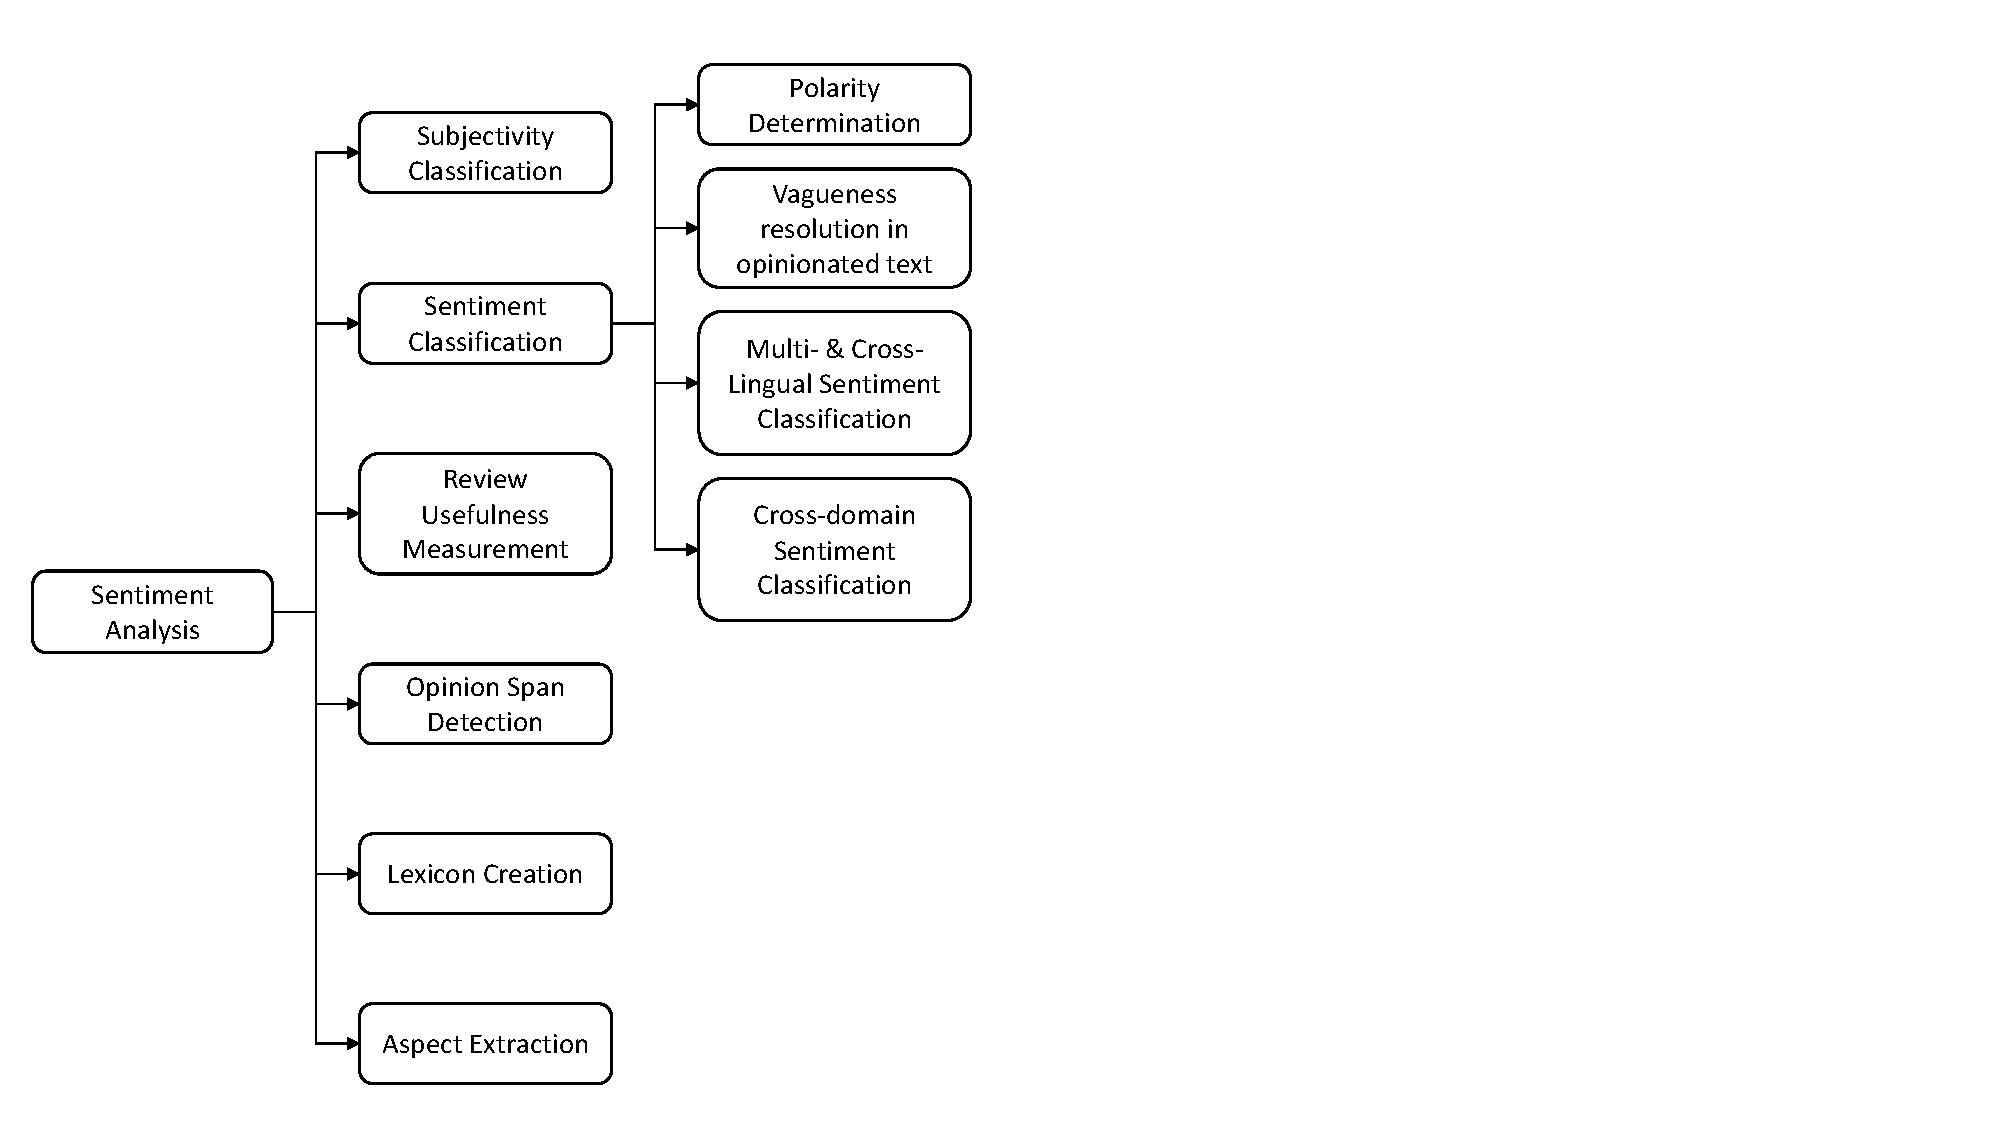
\includegraphics[width=1\textwidth]{figures/sentiment_analysis_tasks}
  \caption{Sentiment analysis tasks.}
  \label{fig:sentiment_analysis_tasks}
\end{figure}

Depending on the problem definition, different tasks have been defined related to sentiment analysis. According to \cite{ravi2015survey}, after the revision of more than three hundred papers related to this topic, the survey carried out concludes that the main tasks can be categorized as (a) subjectivity classification, (b) sentiment classification, (c) review usefulness measurement, (d) opinion spam detection, (e) lexicon creation and (f) aspect extraction, as shown in the figure \ref{fig:sentiment_analysis_tasks}. 

\subsubsection{Subjectivity classification}
\label{subsubsection:subject_classification}

According to \cite{montoyo2012subjectivity}, subjectivity classification aims to determine the "private state" of the author of a text. The Subjectivity analysis is the process of distinguish objective language from the opinion oriented. Even though there is much less literature about this field compared to other \acrshort{sa} task, it has proven to be more difficult than determine the measuring the polarity of a document and, thus, improvements achieved in this field will positively impact on sentiment classification.

\subsubsection{Sentiment classification}
\label{subsubsection:sentiment_classification}

Sentiment classification consist in determine the orientation of a sentiment of a given text into two or more classes. This classification has been performed in multiple classes, such as, binary (positive or negative), ternary (positive, neutral and negative), n-ary, \cite{nakov2016semeval}, among others.

\subsubsection{Review usefulness measurement}
\label{subsubsection:review_usefulness_measurement}

TODO

\subsubsection{Opinion spam detection}
\label{subsubsection:opinion_spam_detection}

TODO

\subsubsection{Lexicon creation}
\label{subsubsection:lexicon_creation}

TODO

\subsubsection{Aspect extraction}
\label{subsubsection:aspect_extraction}

TODO

To solve all these problems in the most efficient way, multiple approaches have been conducted, such as \cite{tripathy2016classification} ; \cite{mullen2004sentiment} or \cite{pouransari2014deep}. The figure \ref{fig:sentiment_analysis_approaches} illustrates which techniques have been used for each previously named categories.

\begin{figure}[!htp]
  \center
  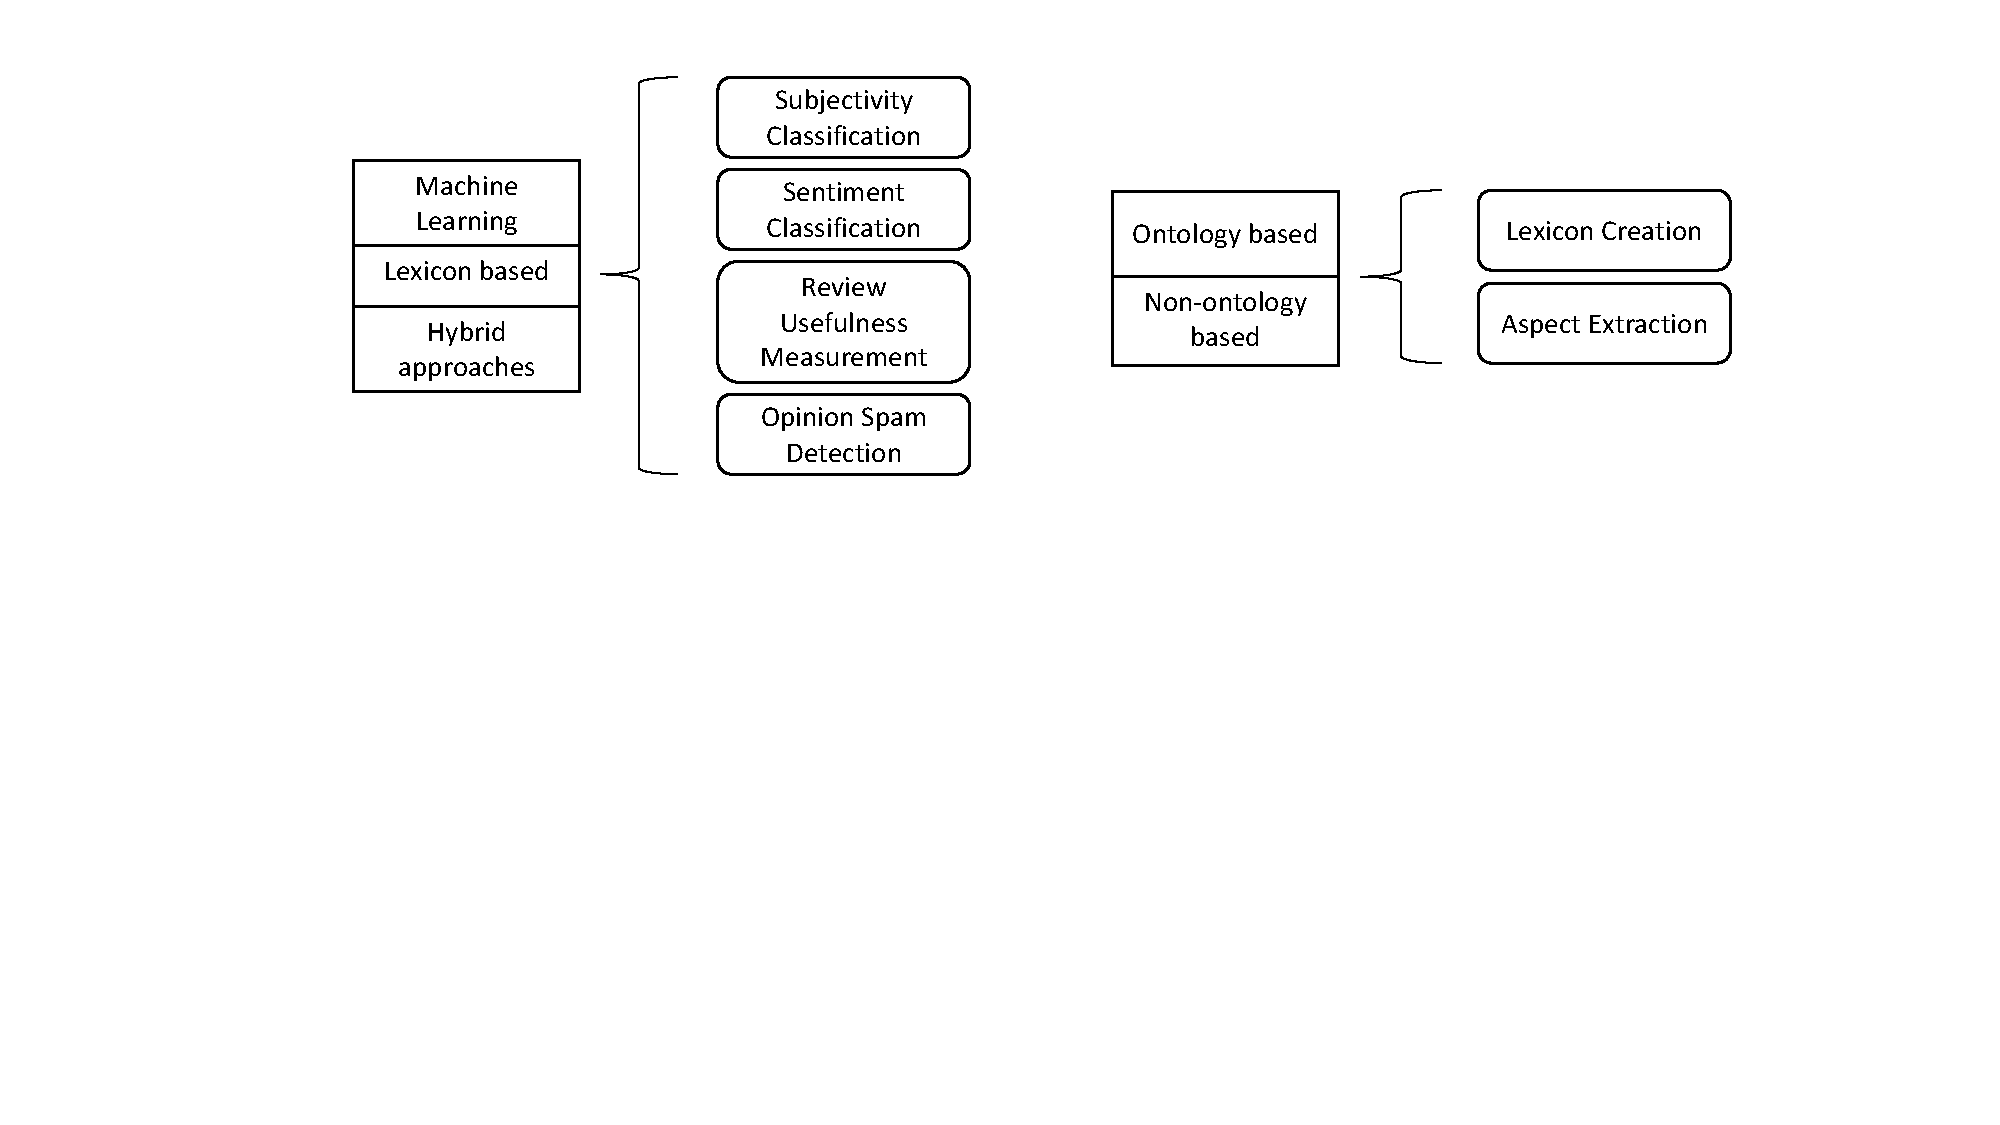
\includegraphics[width=0.9\textwidth]{figures/sentiment_analysis_approaches}
  \caption{Sentiment analysis approaches for each task.}
  \label{fig:sentiment_analysis_approaches}
\end{figure}

\FloatBarrier

\subsection{Techniques}
\label{subsec:sentiment_analysis_techniques}

TODO\cite{thakkar2015approaches}

\begin{figure}[!htp]
  \center
  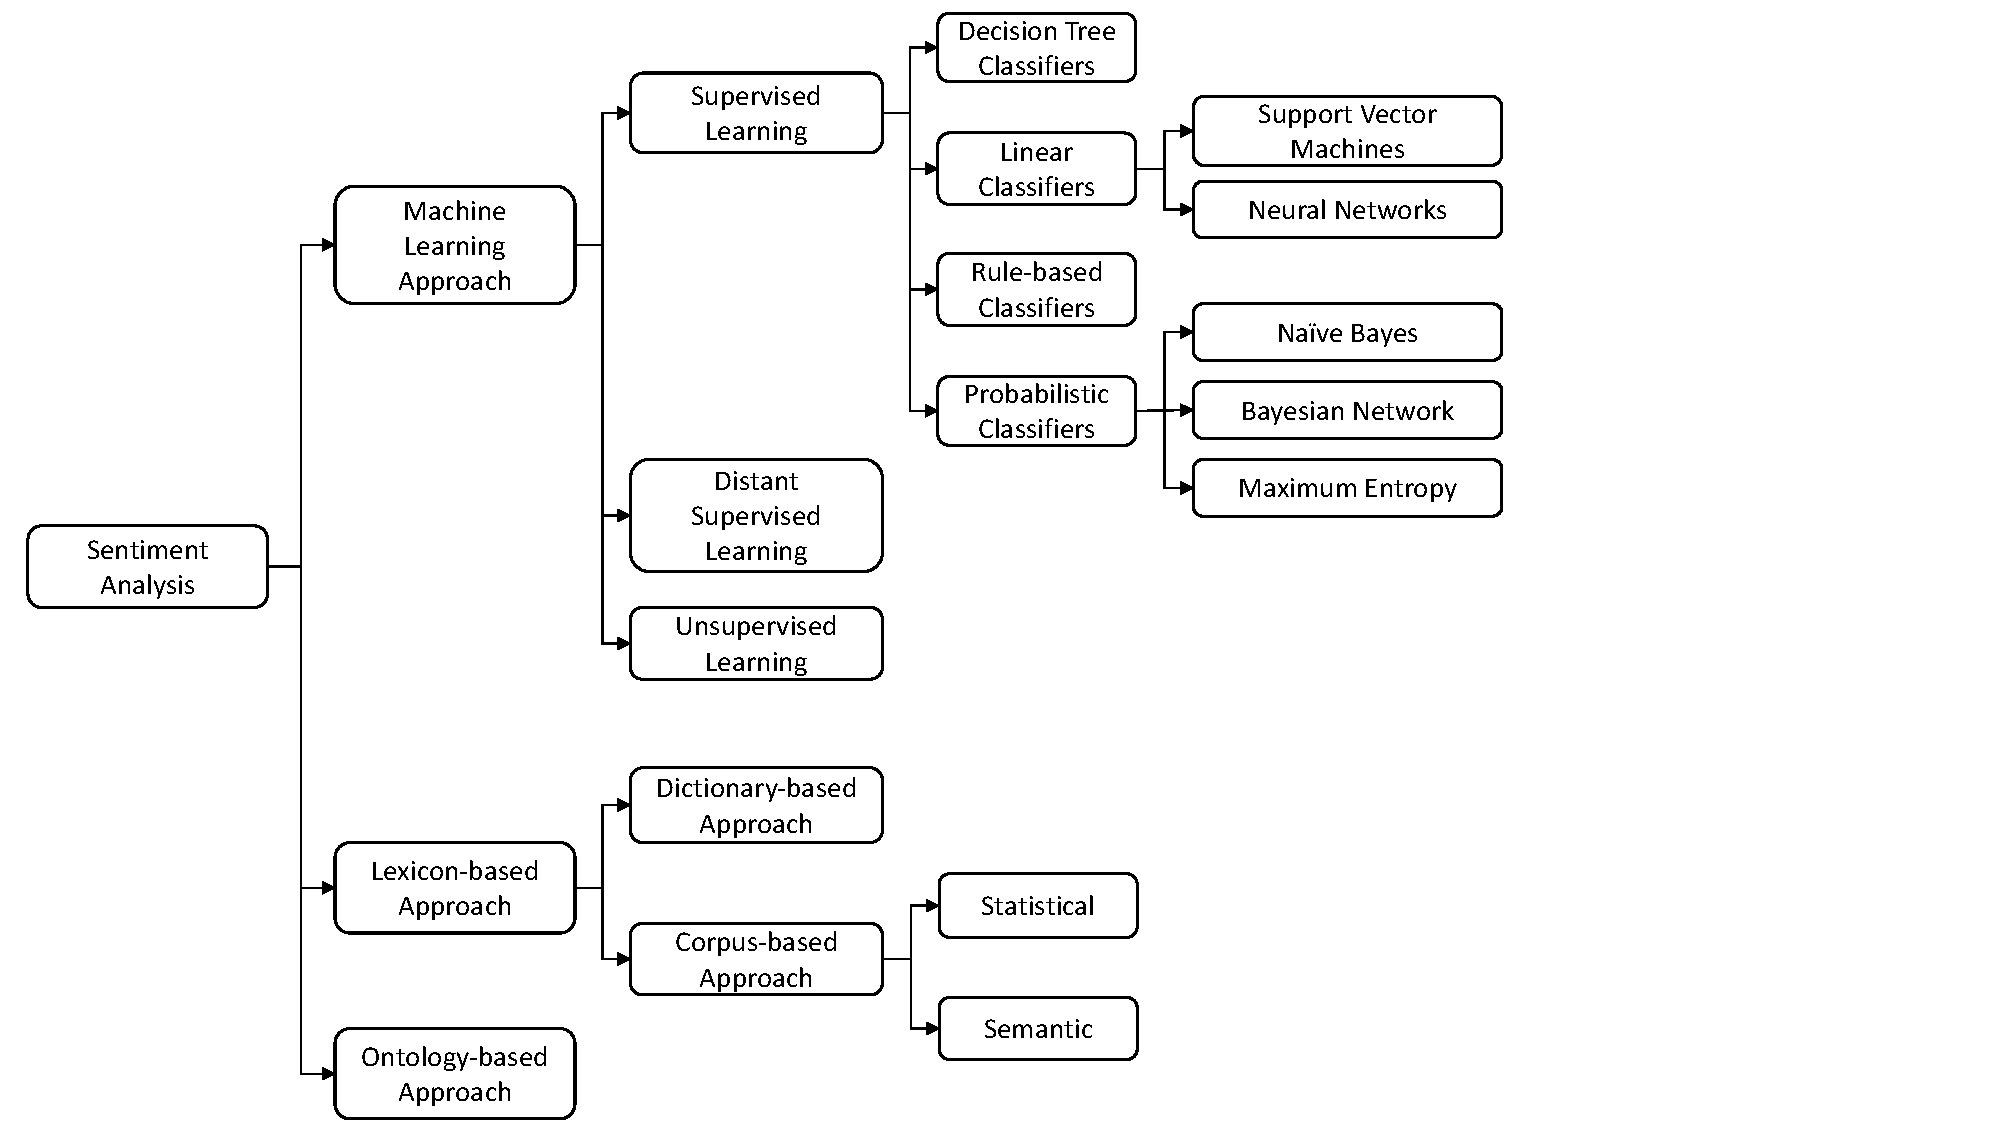
\includegraphics[width=1\textwidth]{figures/sentiment_analysis_techniques}
  \caption{Sentiment analysis techniques\cite{medhat2014sentiment}.}
  \label{fig:sentiment_analysis_techniques}
\end{figure}